\begin{figure}[!htbp]
    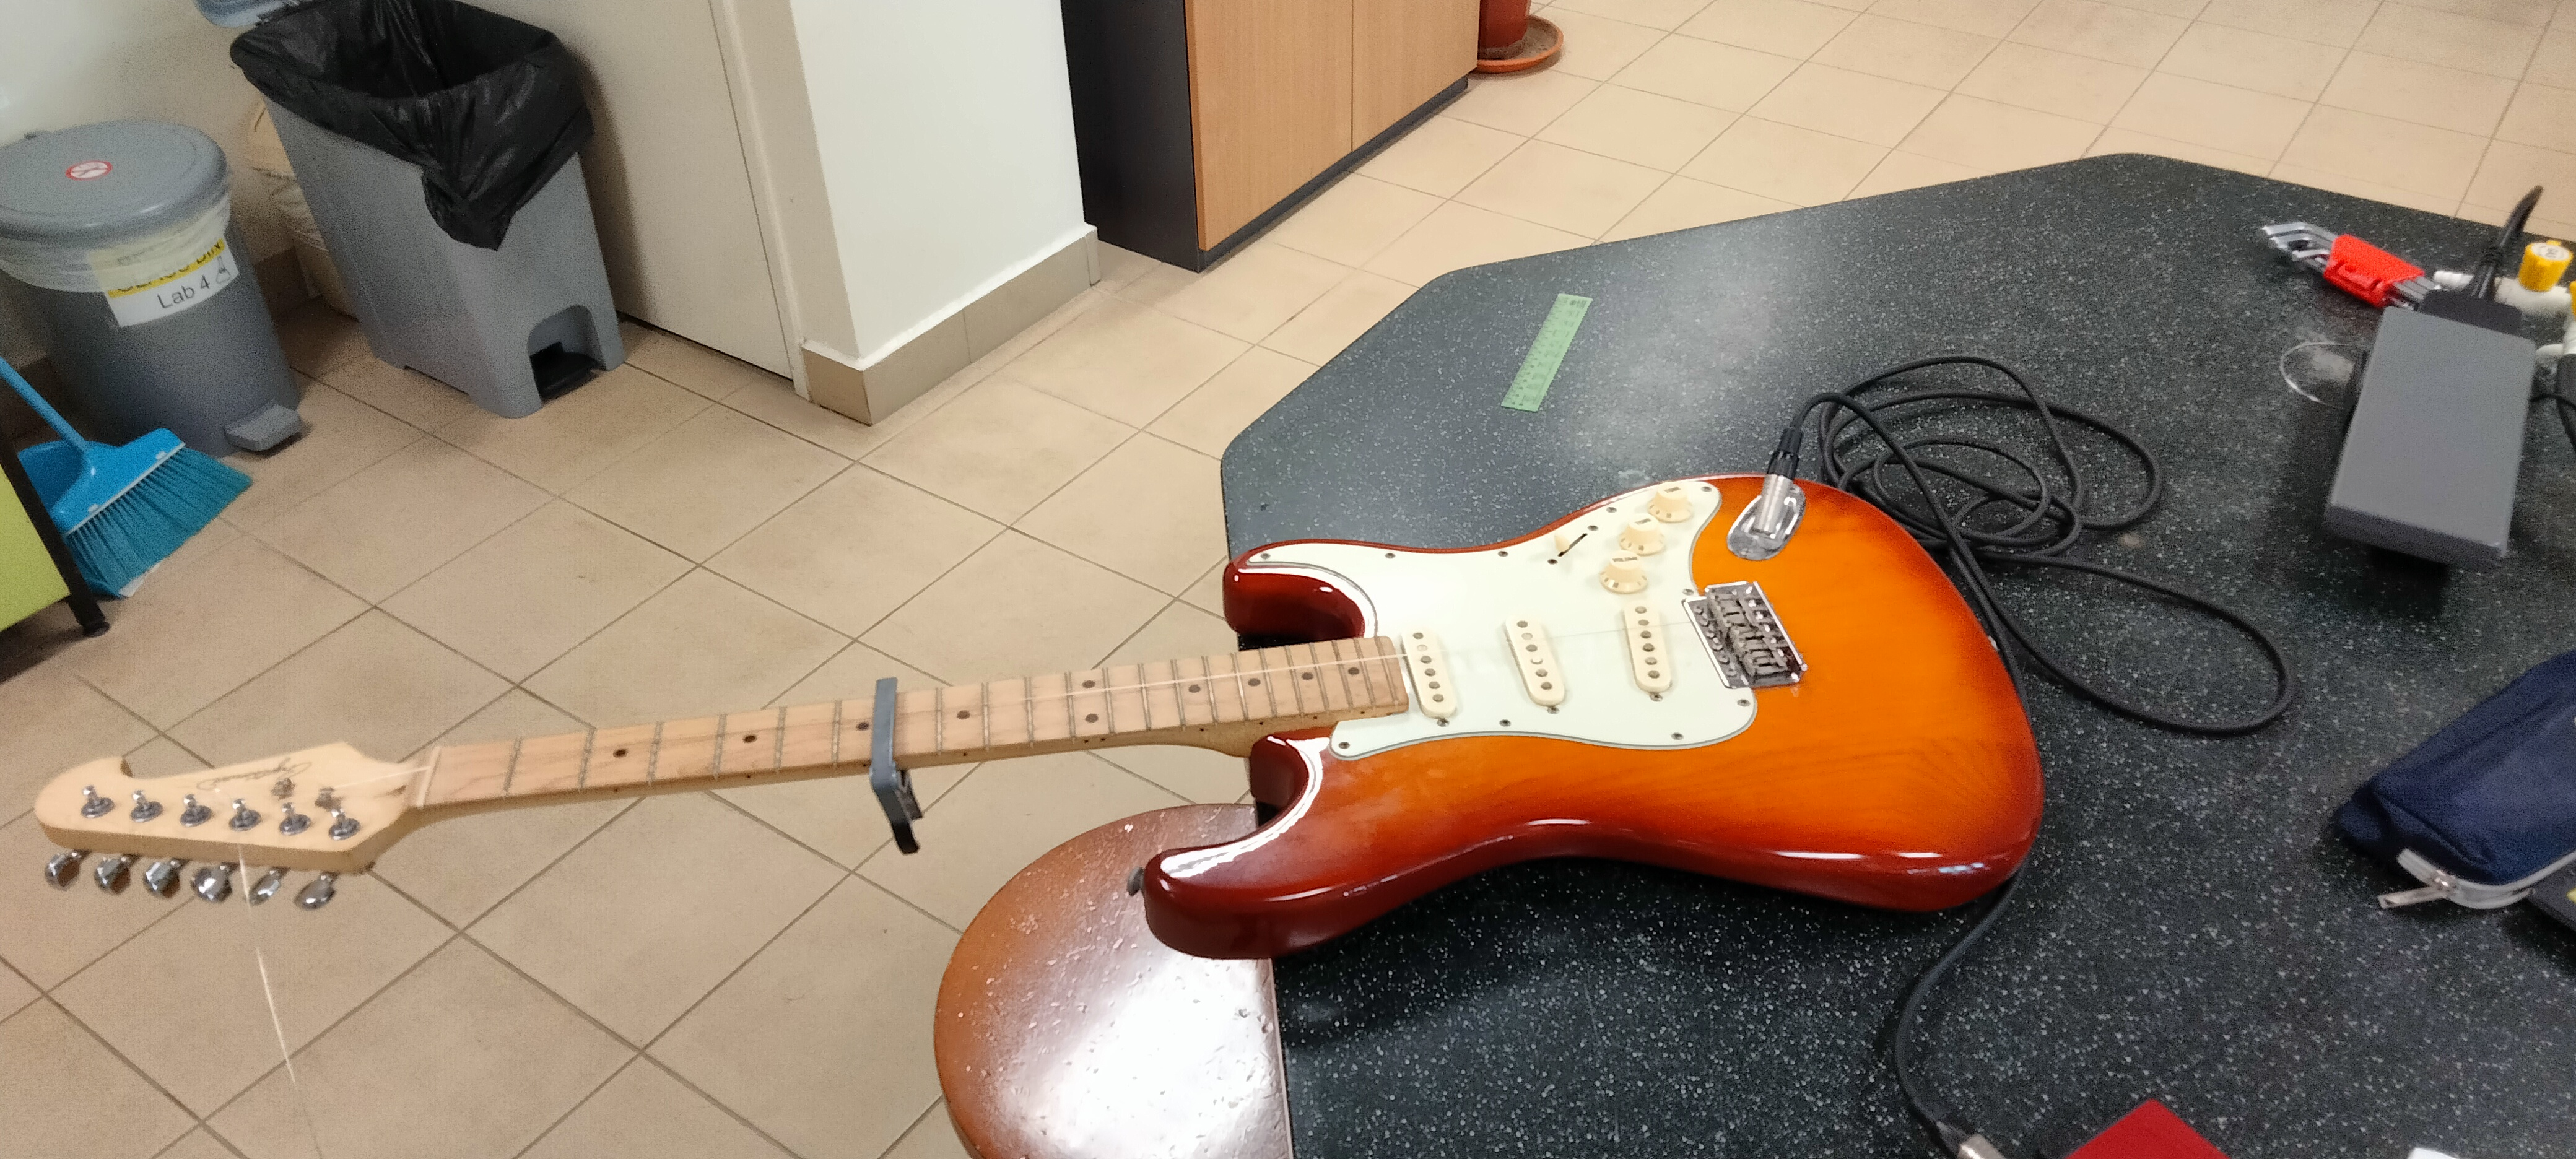
\includegraphics[width = \textwidth]{ee/experiment_setup.jpg}
    \caption{My experimental setup. I position the guitar neck outside the table for ease of access to the capo. The numbers correspond to plucking positions} \label{fig4}
\end{figure}
\begin{figure}[!htbp]
    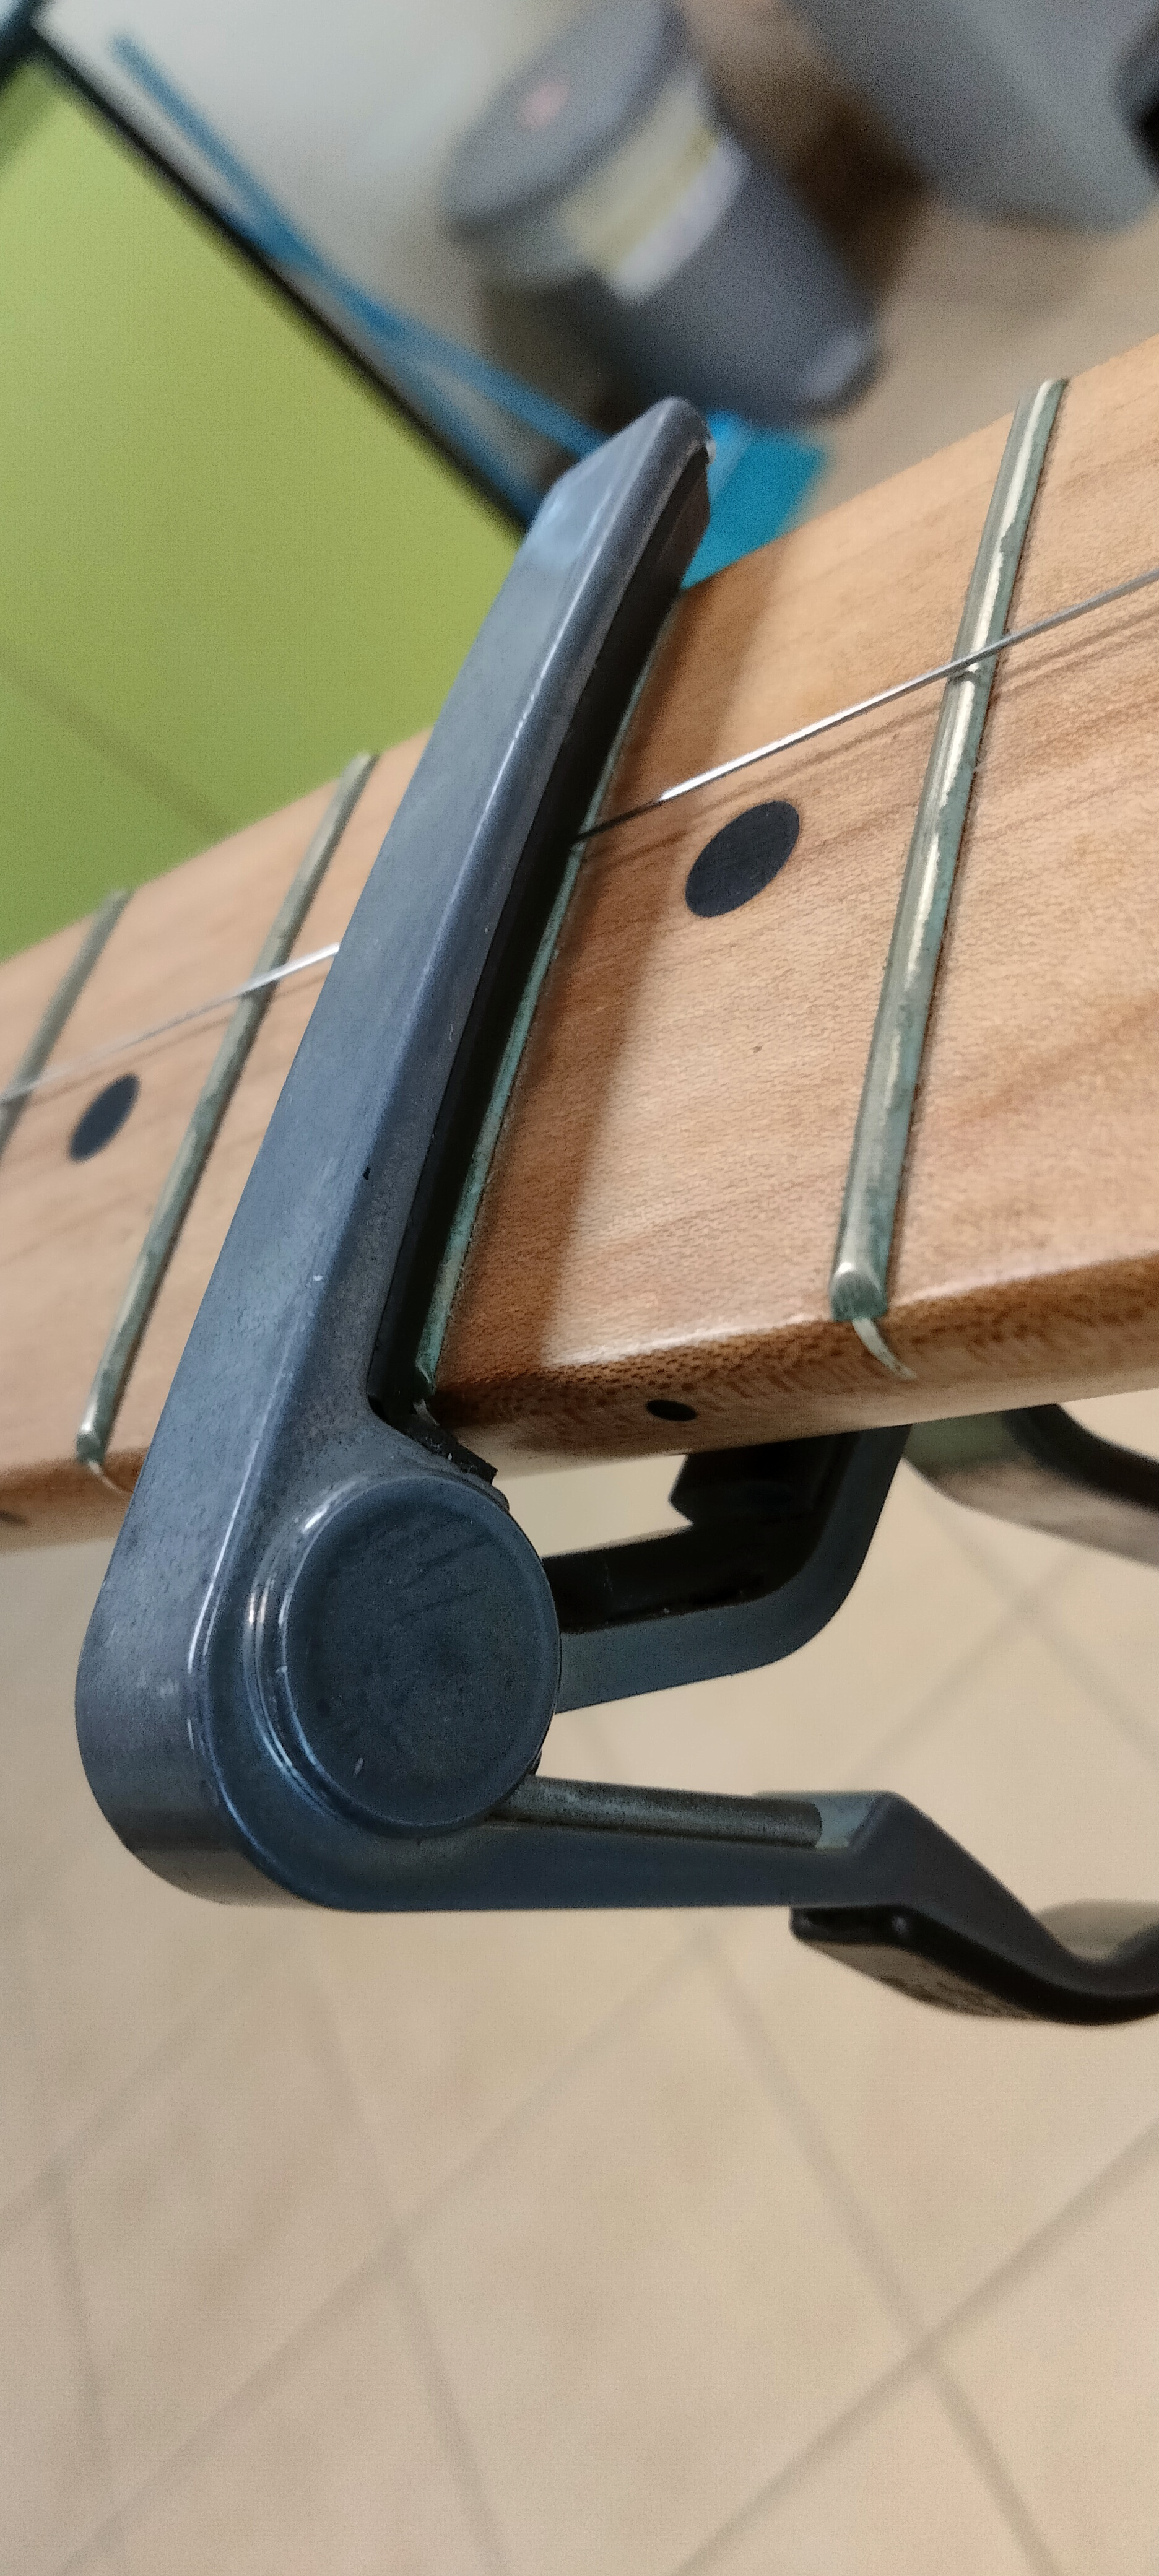
\includegraphics[width = \textwidth]{ee/capo_on_fret.jpg}
    \caption{Close up of capo placement. This ensures consistent pressure and contact with the string and fret} \label{fig5}
\end{figure}
\begin{figure}[!htbp]
    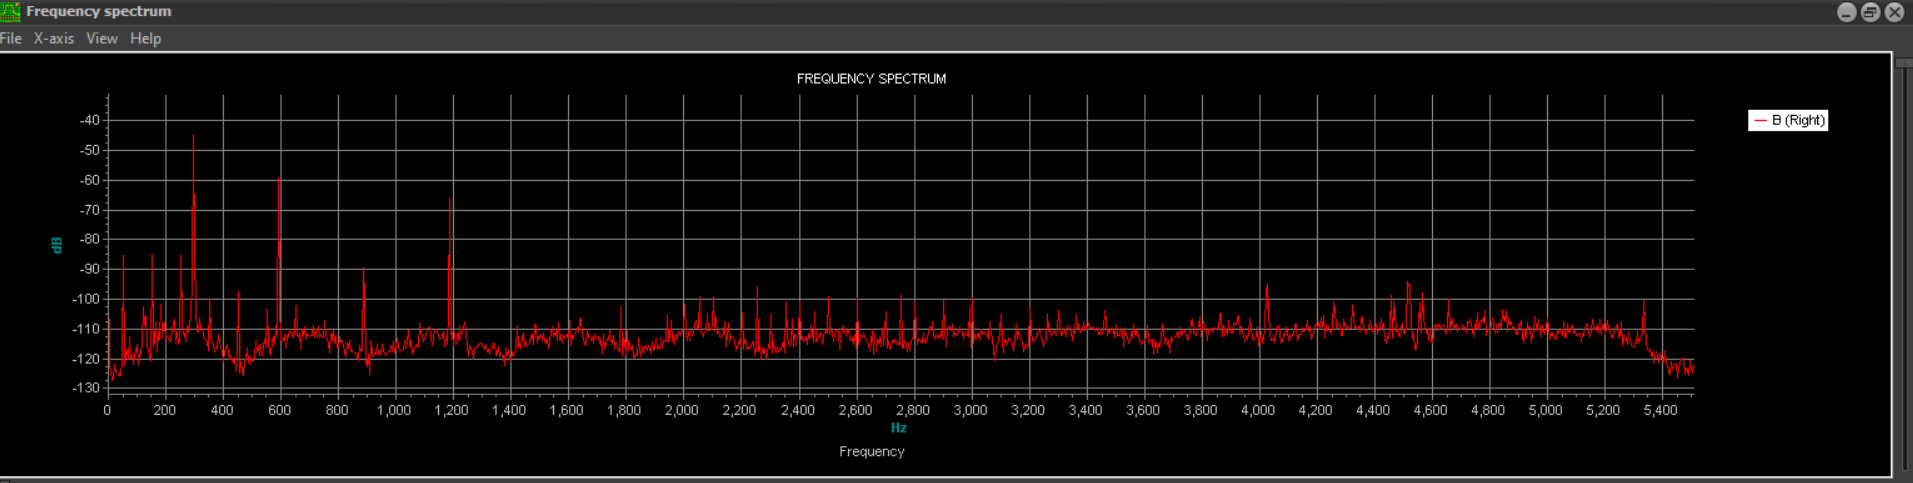
\includegraphics[width = \textwidth]{./ee/freq.png}
    \caption{Frequency spectrum of a note in Visual Analyzer. The peak frequency is circled. This can be zoomed in to accurately read peak value} \label{fig6}
\end{figure}